\documentclass{beamer}
\setbeamertemplate{navigation symbols}{}

\usepackage{beamerthemeshadow}
\usepackage{amsmath}
\usepackage{bm}

\begin{document}
\title{Dynamics of plastic networks of excitatory and inhibitory spiking neurons}  
\author{Clayton Seitz}
\date{\today} 

\begin{frame}[plain]
\titlepage
\end{frame}


\begin{frame}[plain]
\frametitle{Inferring the transfer function from ITC data}

\vspace{0.2in}

\begin{center}
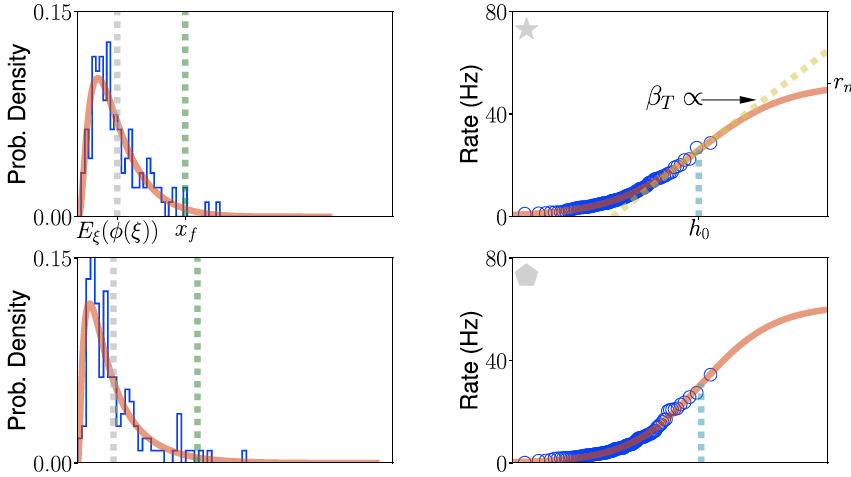
\includegraphics[scale=0.5]{transfer-function}
\end{center}

Measuring the \emph{static} transfer function from novel images assuming that input currents are Gaussian variables

\begin{equation*}
\phi(\bm{\xi}) = \frac{r_{max}}{1 + \exp \beta (\bm{\xi}- \bm{\xi}_{0})}
\end{equation*}


\footnote{\cite{peirera}}
\end{frame}

\begin{frame}[plain]
\frametitle{Inferring the learning rule from ITC data}

\begin{center}
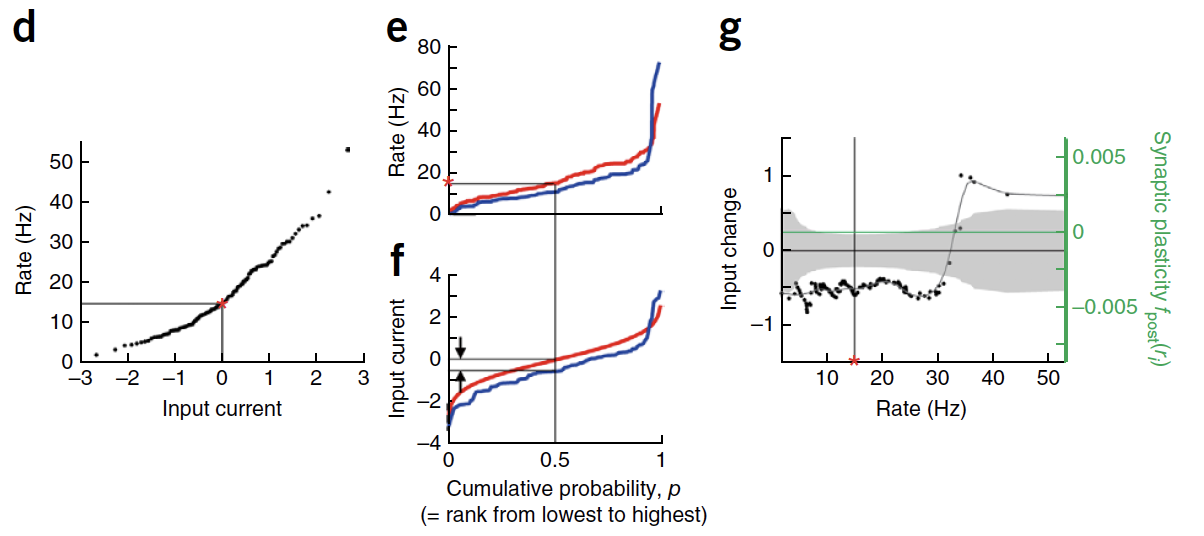
\includegraphics[scale=0.55]{learning-rules}
\end{center}

Inferring the change in input current $\xi_{in}$ from the change in firing rate in {\color{red} novel} relative to {\color{blue} familiar} stimuli

\footnote{\cite{lim}}

\end{frame}

\begin{frame}[plain]
\frametitle{Inferring the learning rule from ITC data}

\begin{center}
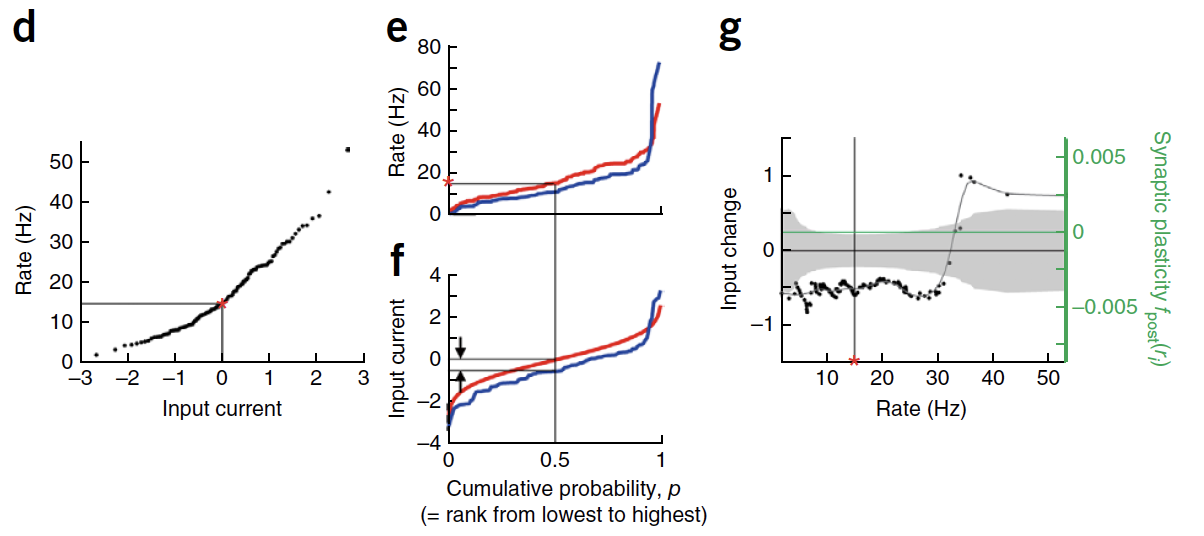
\includegraphics[scale=0.55]{learning-rules}
\end{center}

The change in input current to a neuron can then be read from the firing rate of that neuron when presented a novel stimulus

\begin{align*}
\Delta \xi_{i}(r) \propto (2q + 1 - \tanh (\beta (r-x)))
\end{align*}

\footnote{\cite{lim}}

\end{frame}

\begin{frame}[plain]
\frametitle{A Hebbian update for synaptic weights}

Assuming that $\Delta W_{ij} \propto f(r_{i})g(r_{j})$, the change in input current is related to synaptic plasticity by

\begin{equation*}
\Delta \xi_{i}  \propto  f(r_{i}) \sum_{j} g(r_{j})r_{j}
\end{equation*}

which we have fit from the data as 

\begin{align*}
\Delta \xi_{i}(r) \propto (2q + 1 - \tanh (\beta (r-x)))
\end{align*}

so we can write

\begin{align*}
f(r_{i}) =  \frac{(2q + 1 - \tanh (\beta (r-x)))}{\sum_{j} g(r_{j})r_{j}}\\
\end{align*}


\end{frame}



\begin{frame}[plain]
\frametitle{Presenting novel and familiar stimuli to the network}

\vspace{0.2in}

\begin{center}
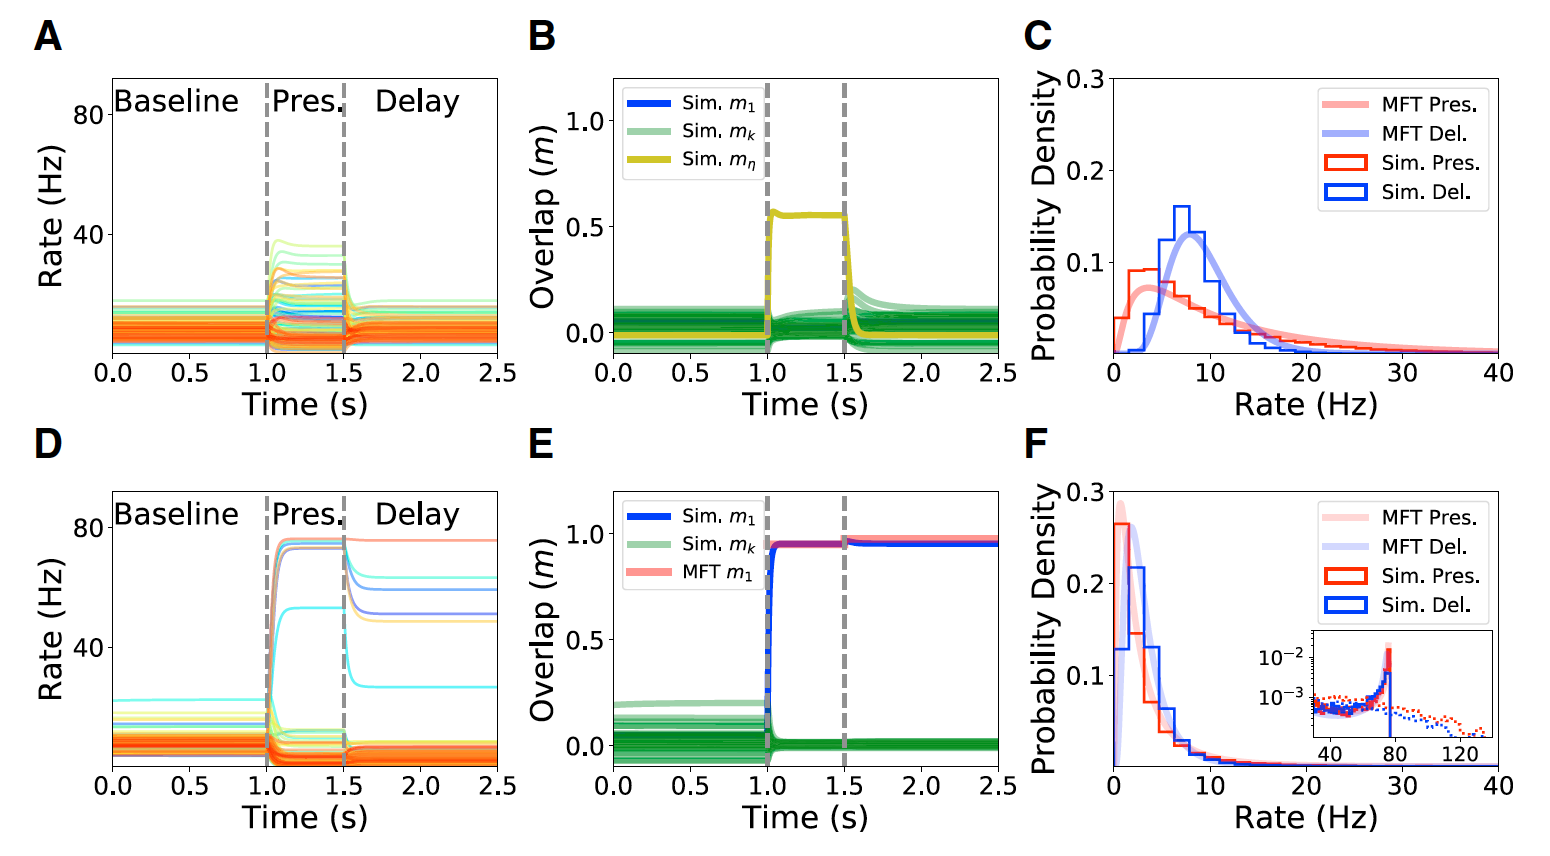
\includegraphics[scale=0.4]{novel-familiar}
\end{center}

\footnote{\cite{peirera}}

\end{frame}




\begin{thebibliography}{99} 
\bibitem[Peirera and Brunel, Neuron. 2018]{peirera}
\bibitem[Lim et al., Nature Neuroscience. 2015]{lim}
\bibitem[J.J. Hopfield PNAS. 1982]{hopfield}
\end{thebibliography}






\end{document}